% Options for packages loaded elsewhere
\PassOptionsToPackage{unicode}{hyperref}
\PassOptionsToPackage{hyphens}{url}
%
\documentclass[
  ignorenonframetext,
]{beamer}
\usepackage{pgfpages}
\setbeamertemplate{caption}[numbered]
\setbeamertemplate{caption label separator}{: }
\setbeamercolor{caption name}{fg=normal text.fg}
\beamertemplatenavigationsymbolsempty
% Prevent slide breaks in the middle of a paragraph
\widowpenalties 1 10000
\raggedbottom
\setbeamertemplate{part page}{
  \centering
  \begin{beamercolorbox}[sep=16pt,center]{part title}
    \usebeamerfont{part title}\insertpart\par
  \end{beamercolorbox}
}
\setbeamertemplate{section page}{
  \centering
  \begin{beamercolorbox}[sep=12pt,center]{part title}
    \usebeamerfont{section title}\insertsection\par
  \end{beamercolorbox}
}
\setbeamertemplate{subsection page}{
  \centering
  \begin{beamercolorbox}[sep=8pt,center]{part title}
    \usebeamerfont{subsection title}\insertsubsection\par
  \end{beamercolorbox}
}
\AtBeginPart{
  \frame{\partpage}
}
\AtBeginSection{
  \ifbibliography
  \else
    \frame{\sectionpage}
  \fi
}
\AtBeginSubsection{
  \frame{\subsectionpage}
}
\usepackage{lmodern}
\usepackage{amsmath}
\usepackage{ifxetex,ifluatex}
\ifnum 0\ifxetex 1\fi\ifluatex 1\fi=0 % if pdftex
  \usepackage[T1]{fontenc}
  \usepackage[utf8]{inputenc}
  \usepackage{textcomp} % provide euro and other symbols
  \usepackage{amssymb}
\else % if luatex or xetex
  \usepackage{unicode-math}
  \defaultfontfeatures{Scale=MatchLowercase}
  \defaultfontfeatures[\rmfamily]{Ligatures=TeX,Scale=1}
\fi
% Use upquote if available, for straight quotes in verbatim environments
\IfFileExists{upquote.sty}{\usepackage{upquote}}{}
\IfFileExists{microtype.sty}{% use microtype if available
  \usepackage[]{microtype}
  \UseMicrotypeSet[protrusion]{basicmath} % disable protrusion for tt fonts
}{}
\makeatletter
\@ifundefined{KOMAClassName}{% if non-KOMA class
  \IfFileExists{parskip.sty}{%
    \usepackage{parskip}
  }{% else
    \setlength{\parindent}{0pt}
    \setlength{\parskip}{6pt plus 2pt minus 1pt}}
}{% if KOMA class
  \KOMAoptions{parskip=half}}
\makeatother
\usepackage{xcolor}
\IfFileExists{xurl.sty}{\usepackage{xurl}}{} % add URL line breaks if available
\IfFileExists{bookmark.sty}{\usepackage{bookmark}}{\usepackage{hyperref}}
\hypersetup{
  pdftitle={MA8701 Advanced methods in statistical inference and learning},
  pdfauthor={Mette Langaas IMF/NTNU},
  hidelinks,
  pdfcreator={LaTeX via pandoc}}
\urlstyle{same} % disable monospaced font for URLs
\newif\ifbibliography
\usepackage{color}
\usepackage{fancyvrb}
\newcommand{\VerbBar}{|}
\newcommand{\VERB}{\Verb[commandchars=\\\{\}]}
\DefineVerbatimEnvironment{Highlighting}{Verbatim}{commandchars=\\\{\}}
% Add ',fontsize=\small' for more characters per line
\usepackage{framed}
\definecolor{shadecolor}{RGB}{248,248,248}
\newenvironment{Shaded}{\begin{snugshade}}{\end{snugshade}}
\newcommand{\AlertTok}[1]{\textcolor[rgb]{0.94,0.16,0.16}{#1}}
\newcommand{\AnnotationTok}[1]{\textcolor[rgb]{0.56,0.35,0.01}{\textbf{\textit{#1}}}}
\newcommand{\AttributeTok}[1]{\textcolor[rgb]{0.77,0.63,0.00}{#1}}
\newcommand{\BaseNTok}[1]{\textcolor[rgb]{0.00,0.00,0.81}{#1}}
\newcommand{\BuiltInTok}[1]{#1}
\newcommand{\CharTok}[1]{\textcolor[rgb]{0.31,0.60,0.02}{#1}}
\newcommand{\CommentTok}[1]{\textcolor[rgb]{0.56,0.35,0.01}{\textit{#1}}}
\newcommand{\CommentVarTok}[1]{\textcolor[rgb]{0.56,0.35,0.01}{\textbf{\textit{#1}}}}
\newcommand{\ConstantTok}[1]{\textcolor[rgb]{0.00,0.00,0.00}{#1}}
\newcommand{\ControlFlowTok}[1]{\textcolor[rgb]{0.13,0.29,0.53}{\textbf{#1}}}
\newcommand{\DataTypeTok}[1]{\textcolor[rgb]{0.13,0.29,0.53}{#1}}
\newcommand{\DecValTok}[1]{\textcolor[rgb]{0.00,0.00,0.81}{#1}}
\newcommand{\DocumentationTok}[1]{\textcolor[rgb]{0.56,0.35,0.01}{\textbf{\textit{#1}}}}
\newcommand{\ErrorTok}[1]{\textcolor[rgb]{0.64,0.00,0.00}{\textbf{#1}}}
\newcommand{\ExtensionTok}[1]{#1}
\newcommand{\FloatTok}[1]{\textcolor[rgb]{0.00,0.00,0.81}{#1}}
\newcommand{\FunctionTok}[1]{\textcolor[rgb]{0.00,0.00,0.00}{#1}}
\newcommand{\ImportTok}[1]{#1}
\newcommand{\InformationTok}[1]{\textcolor[rgb]{0.56,0.35,0.01}{\textbf{\textit{#1}}}}
\newcommand{\KeywordTok}[1]{\textcolor[rgb]{0.13,0.29,0.53}{\textbf{#1}}}
\newcommand{\NormalTok}[1]{#1}
\newcommand{\OperatorTok}[1]{\textcolor[rgb]{0.81,0.36,0.00}{\textbf{#1}}}
\newcommand{\OtherTok}[1]{\textcolor[rgb]{0.56,0.35,0.01}{#1}}
\newcommand{\PreprocessorTok}[1]{\textcolor[rgb]{0.56,0.35,0.01}{\textit{#1}}}
\newcommand{\RegionMarkerTok}[1]{#1}
\newcommand{\SpecialCharTok}[1]{\textcolor[rgb]{0.00,0.00,0.00}{#1}}
\newcommand{\SpecialStringTok}[1]{\textcolor[rgb]{0.31,0.60,0.02}{#1}}
\newcommand{\StringTok}[1]{\textcolor[rgb]{0.31,0.60,0.02}{#1}}
\newcommand{\VariableTok}[1]{\textcolor[rgb]{0.00,0.00,0.00}{#1}}
\newcommand{\VerbatimStringTok}[1]{\textcolor[rgb]{0.31,0.60,0.02}{#1}}
\newcommand{\WarningTok}[1]{\textcolor[rgb]{0.56,0.35,0.01}{\textbf{\textit{#1}}}}
\usepackage{graphicx}
\makeatletter
\def\maxwidth{\ifdim\Gin@nat@width>\linewidth\linewidth\else\Gin@nat@width\fi}
\def\maxheight{\ifdim\Gin@nat@height>\textheight\textheight\else\Gin@nat@height\fi}
\makeatother
% Scale images if necessary, so that they will not overflow the page
% margins by default, and it is still possible to overwrite the defaults
% using explicit options in \includegraphics[width, height, ...]{}
\setkeys{Gin}{width=\maxwidth,height=\maxheight,keepaspectratio}
% Set default figure placement to htbp
\makeatletter
\def\fps@figure{htbp}
\makeatother
\setlength{\emergencystretch}{3em} % prevent overfull lines
\providecommand{\tightlist}{%
  \setlength{\itemsep}{0pt}\setlength{\parskip}{0pt}}
\setcounter{secnumdepth}{-\maxdimen} % remove section numbering
\ifluatex
  \usepackage{selnolig}  % disable illegal ligatures
\fi

\title{MA8701 Advanced methods in statistical inference and learning}
\subtitle{L7: Random forest, Super Learner, Hyperparameter tuning}
\author{Mette Langaas IMF/NTNU}
\date{20 February, 2021}

\begin{document}
\frame{\titlepage}

\begin{frame}{Ensembles - third act}
\protect\hypertarget{ensembles---third-act}{}
\begin{block}{So far}
\protect\hypertarget{so-far}{}
\textbf{L5}:

\begin{itemize}
\tightlist
\item
  Trees
\item
  Many trees with bootstrap aggregation
\item
  Many trees into a random forest (not finished)
\end{itemize}

\textbf{L6}: with Berent Å. S. Lunde (UiB)

\begin{itemize}
\tightlist
\item
  Boosting
\item
  Xgboost
\item
  Avoiding hyperparameter tuning in xgboost
\end{itemize}
\end{block}
\end{frame}

\begin{frame}
\begin{block}{Outline}
\protect\hypertarget{outline}{}
\begin{itemize}
\tightlist
\item
  Ensembles
\item
  Finishing the random forest from
  \href{http://htmlpreview.github.com/?https://github.com/mettelang/MA8701V2021/blob/main/Part2/L5.html}{L5}
\item
  Super Learner
\item
  Hyperparameter tuning
\end{itemize}

Left for L8: How to use statistical inference to give CI and compare
predictions from different methods.
\end{block}
\end{frame}

\begin{frame}{Ensembles - overview}
\protect\hypertarget{ensembles---overview}{}
(ELS Ch 16.1)

With ensembles we want to build \emph{one prediction model} which
combines the strength of \emph{a collection of models}.

These models may be simple base models - or more elaborate models.

We have studied bagging - where we take a simple average of the
prediction from many models (or majority vote), and the base models can
be trees - or other type of models.

Random forest is a version of bagging, with trees made to be different
(decorrelated).
\end{frame}

\begin{frame}
We have studied boosting, where the models are trained on sequentially
different data - from residuals or gradients of loss functions - and the
ensemble members cast weighted votes. We have in particular looked into
the xgboost variant of boosting, and also evaluated possible parameters
to tune to optimize performance.

In L7 we also look into an ensemble built of elaborate models with the
Super Learner and study some possible methods for tuning
hyperparameters.
\end{frame}

\begin{frame}{Random forest}
\protect\hypertarget{random-forest}{}
(ELS Ch 15) see learning material in L5.
\end{frame}

\begin{frame}{Super Learner}
\protect\hypertarget{super-learner}{}
(References: Le Dell (2015) Section 2.2 and van der Laan et al (2016),
and Polley et al (2011))

The Super Learner or \emph{generalized stacking} is an algorithm that
combines

\begin{itemize}
\tightlist
\item
  multiple, (typically) diverse prediction methods (learning algorithms)
  called \emph{base learners} into a
\item
  a \emph{metalearner} - which can be seen as a \emph{single} method.
\end{itemize}
\end{frame}

\begin{frame}
\begin{block}{Development:}
\protect\hypertarget{development}{}
\begin{itemize}
\tightlist
\item
  1992: stacking introduce for neural nets by Wolpert
\item
  1996: adapted to regression problems by Breiman - but only for one
  type of methods at once (cart with different number of terminal nodes,
  glms with subset selection, ridge regression with different ridge
  penalty parameters)
\item
  2006: proven to have asymptotic theoretical oracle property by van der
  Laan, Polley and Hubbard.
\end{itemize}
\end{block}
\end{frame}

\begin{frame}
\begin{block}{Ingredients:}
\protect\hypertarget{ingredients}{}
\begin{itemize}
\tightlist
\item
  \emph{Training data} (level-zero data) \(O_i=(X_i,Y_i)\) of \(N\)
  i.i.d observations.
\item
  A total of \(L\) \emph{base learning algorithms} \(\Psi^l\) for
  \(l=1,\ldots,L\), each from some algorithmic class and each with a
  specific set of model parameters.
\item
  A \emph{metalearner} \({\bf \Phi}\) is used to find an \emph{optimal
  combination} of the \(L\) base learners.
\end{itemize}
\end{block}
\end{frame}

\begin{frame}
\begin{block}{Algorithm}
\protect\hypertarget{algorithm}{}
\textbf{Step 1: Produce level-one data} \({\bf Z}\)

\begin{enumerate}
[a)]
\item
  Divide the training data \({\bf X}\) randomly into \(V\)
  roughly-equally sized validation folds
  \({\bf X}_{(1)},\ldots,{\bf X}_{(V)}\). \(V\) is often 5 or 10.
\item
  For each base learner \(\Phi^l\) perform \(V\)-fold cross-validation
  to produce prediction.
\end{enumerate}

This gives the level-one data set \({\bf Z}\) consisting prediction of
all the level-zero data - that is a matrix with \(N\) rows and \(L\)
columns.

\textbf{What could the base learners be?}
\end{block}
\end{frame}

\begin{frame}
``Any'' method that produces a prediction - ``all'' types of problems.

\begin{itemize}
\tightlist
\item
  linear regression
\item
  lasso
\item
  cart
\item
  random forest with mtry=value 1
\item
  random forest with mtry=value 2
\item
  xgboost with hyperparameter set 1
\item
  xgboost with hyperparameter set 2
\item
  neural net with hyperparameter set 1
\end{itemize}
\end{frame}

\begin{frame}
\textbf{Step 2: Fit the metalearner}

\begin{enumerate}
[a)]
\tightlist
\item
  The starting point is the level-one prediction data \({\bf Z}\)
  together with the responses \((Y_1,\ldots ,Y_N)\).
\item
  The metalearner is used to estimate the weights given to each base
  learner: \(\hat{Y_i}=\alpha_1 z_{1i}+ \cdots + \alpha_L z_{Li}\).
  (Should probably also involve some link function, so that this may be
  the linear predictor.)
\end{enumerate}

\textbf{What could the metalearner be?}
\end{frame}

\begin{frame}
\begin{itemize}
\tightlist
\item
  the mean (bagging)
\item
  ordinary least squares
\item
  non-negative least squares
\item
  ridge or lasso regression
\item
  1-ROC-AUC
\end{itemize}
\end{frame}

\begin{frame}
(Class notes: Study Figure 3.2 from Polley et al)
\end{frame}

\begin{frame}
\textbf{Step 3: Re-estimate base learners and combine into superlearner
on full training data}

\begin{enumerate}
[a)]
\tightlist
\item
  Fit each of the \(L\) base learners to the full training set.
\item
  The \emph{ensemble fit} consists the \(L\) base learner fits together
  with the metalearner fit.
\end{enumerate}

\textbf{Step 4: Using the ensemble for prediction}

For a new observaton \({\bf x}^*\)

\begin{enumerate}
[a)]
\tightlist
\item
  Use each of the \(L\) base learners to produce a prediction
  \({\bf z}^*\), and
\item
  feed this to the metalearnerfit to produce the final prediction
  \(y^*\).
\end{enumerate}
\end{frame}

\begin{frame}
\begin{block}{The metalearning}
\protect\hypertarget{the-metalearning}{}
\begin{itemize}
\tightlist
\item
  The term \emph{discrete super learner} is used if the base learner
  with the lowest risk (i.e.~CV-error) is selected.
\item
  Since the predictions from multiple base learners may be highly
  correlated - the chosen method should perform well in that case
  (i.e.~ridge and lasso)
\item
  when minimizing the squared loss it has been found that adding a
  non-negativity constraint \(\alpha_l\le 0\) works well
\item
  and also the additivity constraint \(\sum_{l=1}^L \alpha_l=1\) - the
  ensemble is a \emph{convex combination} of the base learners
\item
  non-linear optimization methods may be employed for the metalearner if
  no existing algorithm is available
\item
  historically a regularized linear model has ``mostly'' been used
\item
  For classification the logistic response function can be used on the
  linear combination of base learners (Figure 3.2 Polley).
\end{itemize}
\end{block}
\end{frame}

\begin{frame}
\begin{block}{Examples}
\protect\hypertarget{examples}{}
\begin{block}{Simulations examples}
\protect\hypertarget{simulations-examples}{}
(Class notes: Study Figure 3.3 and Table 3.2 from Polley et al)
\end{block}

\begin{block}{Real data}
\protect\hypertarget{real-data}{}
(Class notes: Study Figure 3.4 and Table 3.3 from Polley et al.~RE=MSE
relative to the linear model OLS.)
\end{block}
\end{block}
\end{frame}

\begin{frame}
\begin{block}{Theoretical result}
\protect\hypertarget{theoretical-result}{}
\begin{itemize}
\tightlist
\item
  Oracle selector: the estimator among all possible weighted
  combinations of the base prediction function that minimizes the risk
  under the \emph{true data generating distribution}.
\item
  The \emph{oracle result} was established for the Super Learner by van
  der Laan et al (2006).
\item
  If the \emph{true prediction function} cannot be represented by a
  combination of the base learners (available), then ``optimal'' will be
  the closest linear combination that would be optimal if the true
  data-generating function was known.
\item
  The oracle result require an \emph{uniformly bounded loss function}.
  Using the convex restriction (sum alphas =1) implies that if each
  based learner is bounded so is the convex combination. In practice:
  truncation of the predicted values to the range of the outcome in the
  training set is sufficient to allow for unbounded loss fuctions (Le
  Dell page 6).
\end{itemize}
\end{block}
\end{frame}

\begin{frame}
\begin{block}{Uncertainty in the ensemble}
\protect\hypertarget{uncertainty-in-the-ensemble}{}
(Class notes: Study ``Road map'' 2 from Polley et al)

\begin{itemize}
\tightlist
\item
  Add an outer (external) cross validation loop (where the super learner
  loop is inside). Suggestion: use 20-fold, especially when small sample
  size.
\item
  Overfitting? Check if the super learner does as well or better than
  any of the base learners in the ensemble.
\item
  Results using \emph{influence functions} for estimation of the
  variance for the Super Learner are based on asymptotic variances in
  the use of \(V\)-fold cross-validation (see Ch 5.3 of Le Dell, 2015)
\end{itemize}
\end{block}
\end{frame}

\begin{frame}[fragile]
\begin{block}{Other issues}
\protect\hypertarget{other-issues}{}
\begin{itemize}
\tightlist
\item
  Many different implementations available, and much work on parallell
  processing and speed and memory efficient execution.
\item
  Super learner implicitly can handle hyperparameter tuning by including
  the same base learner with different model parameter sets in the
  ensemble.
\item
  Speed and memory improvements for large data sets involves
  subsampling, and the R \texttt{subsemble} package is one solution, the
  H2O Ensemble project another.
\end{itemize}
\end{block}
\end{frame}

\begin{frame}[fragile]
\begin{block}{R example}
\protect\hypertarget{r-example}{}
Code is copied from \href{}{Guide to SuperLearner} and the presentation
follows this guide. The data used is the Boston housing dataset from
\texttt{MASS}, but with the median value of a house dichotomized into a
classification problem.

Observe that only 150 of the 560 observations is used (to speed up
things, but of cause that gives less accurate results).

\begin{Shaded}
\begin{Highlighting}[]
\FunctionTok{data}\NormalTok{(Boston, }\AttributeTok{package =} \StringTok{"MASS"}\NormalTok{)}
\CommentTok{\#colSums(is.na(Boston)) \# no missing values}
\NormalTok{outcome }\OtherTok{=}\NormalTok{ Boston}\SpecialCharTok{$}\NormalTok{medv}
\CommentTok{\# Create a dataframe to contain our explanatory variables.}
\NormalTok{data }\OtherTok{=} \FunctionTok{subset}\NormalTok{(Boston, }\AttributeTok{select =} \SpecialCharTok{{-}}\NormalTok{medv)}
\CommentTok{\#Set a seed for reproducibility in this random sampling.}
\FunctionTok{set.seed}\NormalTok{(}\DecValTok{1}\NormalTok{)}
\CommentTok{\# Reduce to a dataset of 150 observations to speed up model fitting.}
\NormalTok{train\_obs }\OtherTok{=} \FunctionTok{sample}\NormalTok{(}\FunctionTok{nrow}\NormalTok{(data), }\DecValTok{150}\NormalTok{)}
\CommentTok{\# X is our training sample.}
\NormalTok{x\_train }\OtherTok{=}\NormalTok{ data[train\_obs, ]}
\CommentTok{\# Create a holdout set for evaluating model performance.}
\CommentTok{\# Note: cross{-}validation is even better than a single holdout sample.}
\NormalTok{x\_holdout }\OtherTok{=}\NormalTok{ data[}\SpecialCharTok{{-}}\NormalTok{train\_obs, ]}
\CommentTok{\# Create a binary outcome variable: towns in which median home value is \textgreater{} 22,000.}
\NormalTok{outcome\_bin }\OtherTok{=} \FunctionTok{as.numeric}\NormalTok{(outcome }\SpecialCharTok{\textgreater{}} \DecValTok{22}\NormalTok{)}
\NormalTok{y\_train }\OtherTok{=}\NormalTok{ outcome\_bin[train\_obs]}
\NormalTok{y\_holdout }\OtherTok{=}\NormalTok{ outcome\_bin[}\SpecialCharTok{{-}}\NormalTok{train\_obs]}
\FunctionTok{table}\NormalTok{(y\_train, }\AttributeTok{useNA =} \StringTok{"ifany"}\NormalTok{)}
\end{Highlighting}
\end{Shaded}

\begin{verbatim}
## y_train
##  0  1 
## 92 58
\end{verbatim}

Then checking out the possible functions and how they differ from their
``original versions''.

\begin{Shaded}
\begin{Highlighting}[]
\FunctionTok{listWrappers}\NormalTok{()}
\end{Highlighting}
\end{Shaded}

\begin{verbatim}
##  [1] "SL.bartMachine"      "SL.bayesglm"         "SL.biglasso"        
##  [4] "SL.caret"            "SL.caret.rpart"      "SL.cforest"         
##  [7] "SL.earth"            "SL.extraTrees"       "SL.gam"             
## [10] "SL.gbm"              "SL.glm"              "SL.glm.interaction" 
## [13] "SL.glmnet"           "SL.ipredbagg"        "SL.kernelKnn"       
## [16] "SL.knn"              "SL.ksvm"             "SL.lda"             
## [19] "SL.leekasso"         "SL.lm"               "SL.loess"           
## [22] "SL.logreg"           "SL.mean"             "SL.nnet"            
## [25] "SL.nnls"             "SL.polymars"         "SL.qda"             
## [28] "SL.randomForest"     "SL.ranger"           "SL.ridge"           
## [31] "SL.rpart"            "SL.rpartPrune"       "SL.speedglm"        
## [34] "SL.speedlm"          "SL.step"             "SL.step.forward"    
## [37] "SL.step.interaction" "SL.stepAIC"          "SL.svm"             
## [40] "SL.template"         "SL.xgboost"         
## [1] "All"
## [1] "screen.corP"           "screen.corRank"        "screen.glmnet"        
## [4] "screen.randomForest"   "screen.SIS"            "screen.template"      
## [7] "screen.ttest"          "write.screen.template"
\end{verbatim}

\begin{Shaded}
\begin{Highlighting}[]
\CommentTok{\# how does SL.glm differ from glm? obsWeight added to easy use the traning fold in the CV and returns a prediction for new observarions}
\NormalTok{SL.glm}
\end{Highlighting}
\end{Shaded}

\begin{verbatim}
## function (Y, X, newX, family, obsWeights, model = TRUE, ...) 
## {
##     if (is.matrix(X)) {
##         X = as.data.frame(X)
##     }
##     fit.glm <- glm(Y ~ ., data = X, family = family, weights = obsWeights, 
##         model = model)
##     if (is.matrix(newX)) {
##         newX = as.data.frame(newX)
##     }
##     pred <- predict(fit.glm, newdata = newX, type = "response")
##     fit <- list(object = fit.glm)
##     class(fit) <- "SL.glm"
##     out <- list(pred = pred, fit = fit)
##     return(out)
## }
## <bytecode: 0x7fec59152f60>
## <environment: namespace:SuperLearner>
\end{verbatim}

\begin{Shaded}
\begin{Highlighting}[]
\CommentTok{\# min and not 1sd used, again obsWeights, make sure model matrix correctly specified}
\NormalTok{SL.glmnet}
\end{Highlighting}
\end{Shaded}

\begin{verbatim}
## function (Y, X, newX, family, obsWeights, id, alpha = 1, nfolds = 10, 
##     nlambda = 100, useMin = TRUE, loss = "deviance", ...) 
## {
##     .SL.require("glmnet")
##     if (!is.matrix(X)) {
##         X <- model.matrix(~-1 + ., X)
##         newX <- model.matrix(~-1 + ., newX)
##     }
##     fitCV <- glmnet::cv.glmnet(x = X, y = Y, weights = obsWeights, 
##         lambda = NULL, type.measure = loss, nfolds = nfolds, 
##         family = family$family, alpha = alpha, nlambda = nlambda, 
##         ...)
##     pred <- predict(fitCV, newx = newX, type = "response", s = ifelse(useMin, 
##         "lambda.min", "lambda.1se"))
##     fit <- list(object = fitCV, useMin = useMin)
##     class(fit) <- "SL.glmnet"
##     out <- list(pred = pred, fit = fit)
##     return(out)
## }
## <bytecode: 0x7fec5900d388>
## <environment: namespace:SuperLearner>
\end{verbatim}

The fitting lasso to check what is being done. The default metalearner
is ``method.NNLS'' (both for regression and two-class classification -
probably then for linear predictor NNLS?).

\begin{Shaded}
\begin{Highlighting}[]
\FunctionTok{set.seed}\NormalTok{(}\DecValTok{1}\NormalTok{)}
\NormalTok{sl\_lasso}\OtherTok{=}\FunctionTok{SuperLearner}\NormalTok{(}\AttributeTok{Y=}\NormalTok{y\_train, }\AttributeTok{X=}\NormalTok{x\_train,}\AttributeTok{family=}\FunctionTok{binomial}\NormalTok{(),}\AttributeTok{SL.library=}\StringTok{"SL.glmnet"}\NormalTok{)}
\NormalTok{sl\_lasso}
\end{Highlighting}
\end{Shaded}

\begin{verbatim}
## 
## Call:  
## SuperLearner(Y = y_train, X = x_train, family = binomial(), SL.library = "SL.glmnet") 
## 
## 
## 
##                     Risk Coef
## SL.glmnet_All 0.08484849    1
\end{verbatim}

\begin{Shaded}
\begin{Highlighting}[]
\CommentTok{\#str(sl\_lasso)}
\NormalTok{sl\_lasso}\SpecialCharTok{$}\NormalTok{cvRisk}
\end{Highlighting}
\end{Shaded}

\begin{verbatim}
## SL.glmnet_All 
##    0.08484849
\end{verbatim}

Now use lasso and randomforest, and also add the average of ys just as
the benchmark.

\begin{Shaded}
\begin{Highlighting}[]
\FunctionTok{set.seed}\NormalTok{(}\DecValTok{1}\NormalTok{)}
\NormalTok{sl}\OtherTok{=}\FunctionTok{SuperLearner}\NormalTok{(}\AttributeTok{Y=}\NormalTok{y\_train, }\AttributeTok{X=}\NormalTok{x\_train,}\AttributeTok{family=}\FunctionTok{binomial}\NormalTok{(),}\AttributeTok{SL.library=}\FunctionTok{c}\NormalTok{(}\StringTok{"SL.mean"}\NormalTok{,}\StringTok{"SL.glmnet"}\NormalTok{,}\StringTok{"SL.randomForest"}\NormalTok{))}
\NormalTok{sl}
\end{Highlighting}
\end{Shaded}

\begin{verbatim}
## 
## Call:  
## SuperLearner(Y = y_train, X = x_train, family = binomial(), SL.library = c("SL.mean",  
##     "SL.glmnet", "SL.randomForest")) 
## 
## 
##                           Risk     Coef
## SL.mean_All         0.23773937 0.000000
## SL.glmnet_All       0.08725786 0.134252
## SL.randomForest_All 0.07213058 0.865748
\end{verbatim}

\begin{Shaded}
\begin{Highlighting}[]
\NormalTok{sl}\SpecialCharTok{$}\NormalTok{times}\SpecialCharTok{$}\NormalTok{everything}
\end{Highlighting}
\end{Shaded}

\begin{verbatim}
##    user  system elapsed 
##   3.086   0.063   3.156
\end{verbatim}

Our ensemble give weight 0.13 to lasso and 0.86 to the random forest.
(The guide used a different implementation of the random forest called
ranger, and got 0.02 and 0.98.)

Predict on the part of the dataset not used for the training.

\begin{Shaded}
\begin{Highlighting}[]
\NormalTok{pred}\OtherTok{=}\FunctionTok{predict}\NormalTok{(sl,}\AttributeTok{x\_holdout=}\NormalTok{x\_holdout,}\AttributeTok{onlySL=}\ConstantTok{TRUE}\NormalTok{)}
\FunctionTok{str}\NormalTok{(pred)}
\end{Highlighting}
\end{Shaded}

\begin{verbatim}
## List of 2
##  $ pred           : num [1:150, 1] 0.3029 0.07 0.97847 0.00726 0.00523 ...
##   ..- attr(*, "dimnames")=List of 2
##   .. ..$ : chr [1:150] "505" "324" "167" "129" ...
##   .. ..$ : NULL
##  $ library.predict: num [1:150, 1:3] 0.387 0.387 0.387 0.387 0.387 ...
##   ..- attr(*, "dimnames")=List of 2
##   .. ..$ : chr [1:150] "505" "324" "167" "129" ...
##   .. ..$ : chr [1:3] "SL.mean_All" "SL.glmnet_All" "SL.randomForest_All"
\end{verbatim}

\begin{Shaded}
\begin{Highlighting}[]
\FunctionTok{summary}\NormalTok{(pred}\SpecialCharTok{$}\NormalTok{pred)}
\end{Highlighting}
\end{Shaded}

\begin{verbatim}
##        V1           
##  Min.   :0.0003034  
##  1st Qu.:0.0183955  
##  Median :0.1135270  
##  Mean   :0.3855066  
##  3rd Qu.:0.9036164  
##  Max.   :0.9955802
\end{verbatim}

\begin{Shaded}
\begin{Highlighting}[]
\FunctionTok{summary}\NormalTok{(pred}\SpecialCharTok{$}\NormalTok{library.predict)}
\end{Highlighting}
\end{Shaded}

\begin{verbatim}
##   SL.mean_All     SL.glmnet_All       SL.randomForest_All
##  Min.   :0.3867   Min.   :0.0000014   Min.   :0.0000     
##  1st Qu.:0.3867   1st Qu.:0.0244935   1st Qu.:0.0160     
##  Median :0.3867   Median :0.2063204   Median :0.1020     
##  Mean   :0.3867   Mean   :0.3866667   Mean   :0.3853     
##  3rd Qu.:0.3867   3rd Qu.:0.8169726   3rd Qu.:0.9123     
##  Max.   :0.3867   Max.   :0.9997871   Max.   :0.9980
\end{verbatim}

Add now an external cross-validation loop - only using the training
data. Here the default \(V=10\) is used for the inner loop, and we set
the value for the outer loop (here \(V=3\) for speed).

\begin{Shaded}
\begin{Highlighting}[]
\FunctionTok{system.time}\NormalTok{(\{cv\_sl}\OtherTok{=}\FunctionTok{CV.SuperLearner}\NormalTok{(}\AttributeTok{Y=}\NormalTok{y\_train, }\AttributeTok{X=}\NormalTok{x\_train,}\AttributeTok{V=}\DecValTok{3}\NormalTok{,}\AttributeTok{family=}\FunctionTok{binomial}\NormalTok{(),}\AttributeTok{SL.library=}\FunctionTok{c}\NormalTok{(}\StringTok{"SL.mean"}\NormalTok{,}\StringTok{"SL.glmnet"}\NormalTok{,}\StringTok{"SL.randomForest"}\NormalTok{))\})}
\end{Highlighting}
\end{Shaded}

\begin{verbatim}
##    user  system elapsed 
##   8.404   0.166   8.583
\end{verbatim}

\begin{Shaded}
\begin{Highlighting}[]
\FunctionTok{summary}\NormalTok{(cv\_sl)}
\end{Highlighting}
\end{Shaded}

\begin{verbatim}
## 
## Call:  
## CV.SuperLearner(Y = y_train, X = x_train, V = 3, family = binomial(), SL.library = c("SL.mean",  
##     "SL.glmnet", "SL.randomForest")) 
## 
## Risk is based on: Mean Squared Error
## 
## All risk estimates are based on V =  3 
## 
##            Algorithm      Ave        se      Min     Max
##        Super Learner 0.091052 0.0154191 0.056368 0.13943
##          Discrete SL 0.095636 0.0168328 0.056368 0.15197
##          SL.mean_All 0.242933 0.0096227 0.227600 0.26920
##        SL.glmnet_All 0.100032 0.0166562 0.062690 0.15197
##  SL.randomForest_All 0.078871 0.0119605 0.056368 0.10168
\end{verbatim}

See the guide for more information on running multiple versions of one
base learner, and parallellisation.
\end{block}
\end{frame}

\begin{frame}{Choosing hyperparameters}
\protect\hypertarget{choosing-hyperparameters}{}
\begin{itemize}
\tightlist
\item
  What are \emph{hyperparameters}?
\item
  Which hyperparameters have we encountered in the course so far?
\end{itemize}
\end{frame}

\begin{frame}
\emph{Hyperparameters} are parameters than cannot be directly estimated
from data. This may be model parameters (the \(\lambda\) in lasso) or
parameters that influence the fitting of the model (e.g.~related to some
optimization algorithm).

We have already studied hyperparameter tuning for the lasso, ridge,
elastic net, random forest, and boosting - with the use of
cross-validation of some loss function for a predefined set of
hyperparameter values.

The use of ensembles like the Super Learner may be seen as an
alternative to hyperparameter tuning.
\end{frame}

\begin{frame}
Overview of advices from Berent Å.S. Lunde on tuning parameters in
xbgoost (written out after the lecture and approved by Berent):

\textbf{Ways to speed-up computation:}

\begin{itemize}
\tightlist
\item
  Higher learning-rate, then tune the number of boosting iterations.
\item
  When tuning, do not use too high k in k-fold CV (for both speed and
  also to avoid high variance), or drop CV and use a validation set.
\item
  Speedups with histogram algorithms of order \(n\) (avoid exact
  enumeration of all splits, nlogn).
\item
  Use sparsity when possible!
\end{itemize}
\end{frame}

\begin{frame}
\textbf{Comments on hyperparameters:}

\begin{itemize}
\tightlist
\item
  Learning rate (eta in xgb): Set as low as computation times allow.
  Typically in between \(0.01\) and \(0.1\) is sufficient.
\item
  Number of trees (boosting iterations): Very much affected by the
  learning rate. Most important parameter to tune, given a learning
  rate. @ Maximum depth of trees: start low, then increase. High values
  takes significantly longer to train. Think about the problem, and the
  number of possible interaction effects. If max-depth = J, then
  interactions among J-1 features is possible. How much is needed?
\item
  Gamma: Very traditional tree-hyperparameter to tune. Tune.
\item
  Colsampling for tree is usually sufficient.
\item
  subsample: in 0.5-0.9
\item
  Min child weight: Something I usually do not think about. Default=1
  (low) works. For me
\end{itemize}

Every problem is different, and there will exist exceptions to the above
guidelines. \emph{I look forward to a world without hyperparameters.}
(Berent Å.S. Lunde)
\end{frame}

\begin{frame}
The hyperparameters may be continuous (penalty parameter), discrete
(number of layers in a neural network, applying early stopping or not)
or categorical (choose between different optimizers).

The choice of hyperparameters is important, and will often directly
affect the model complexity, and unwise choices may lead to overfitting.
\end{frame}

\begin{frame}
Hyperparametertuning is performed using a separate validation set or by
cross-validation. Different loss functions or selection criteria may be
used (MSE, AUC, misclassification rate, \ldots).

The hyperparameter tuning is often referred to as a black-box
optimization because we (usually) only calculate loss function values
(with CV) and do not get to compute gradients.

What may be challenges with hyperparameter optimization?
\end{frame}

\begin{frame}
Some challenges with hyperparameter optimization (Feurer and Hutter,
Ch1):

\begin{itemize}
\tightlist
\item
  expensive evaluation of the model under study (large networks, large
  data sets)
\item
  unclear which of possibly many hyperparameters that need to be
  selected carefully (refer to the discussion for xgboost)
\item
  gradient of selection criterion with respect to the hyperparameters
  not (generally) available, and criterion not convex or smooth in the
  hyperparameters
\item
  and the need for external validation or CV
\end{itemize}
\end{frame}

\begin{frame}
There exist many ways to \emph{group} methods for hyperparameter tuning.
One way to look at this is (Kuhn and Silge, 2021, Ch 12)

\begin{itemize}
\tightlist
\item
  grid search: specify a set of possible values a priori and investigate
  only these values, choose the value where the chosen selection
  criterion is optimal. This is also called ``model free methods''.
\item
  iterative search: start with a set of values, fit/evaluate some
  (surrogate) model (might also be the loss function), and based on this
  choose new values to evaluate next.
\end{itemize}

For grid search also methods for \emph{speeding up calculations} exists
- for example by stopping evaluation at a grid point where the loss is
seen to be high after some CV-folds, for example the method of
\emph{racing} described by Kuhn and Silge, Ch 13.4.
\end{frame}

\begin{frame}
(Class notes: see example from Kuhn and Silge, 2021, Spacefilling grid
vs global search)
\end{frame}

\begin{frame}
\begin{block}{Surrogate methods}
\protect\hypertarget{surrogate-methods}{}
We will look at two types of surrogate models: Bayesian regression with
Gaussian processes (in Bayesian optimization) and regression-type models
in response surface methods (presented by group 2).
\end{block}

\begin{block}{Bayesian optimization}
\protect\hypertarget{bayesian-optimization}{}
Bayesian optimization is an iterative method - where we start with
evaluating some loss function at some predefined set of points in the
hyperparameter space. New position in the hyperparameter space are
chosen iteratively.

Two key ingredients:

\begin{itemize}
\tightlist
\item
  a surrogate model (we will only look at Bayesian regression with
  Gaussian processes) to fit to the observed values of the loss function
  in the hyperparameter space
\item
  an \emph{acquisition} function to decide a new point in the
  hyperparameter space to evaluate next
\end{itemize}
\end{block}
\end{frame}

\begin{frame}
Underlying idea: given some ``observations'' in the hyperparameter
space, the task is to decide where to place a new point. We should try a
point where:

\begin{itemize}
\tightlist
\item
  we expect a good value and/or
\item
  we have little information so far
\end{itemize}

To do that we need information on both expected value \emph{and}
variance - or preferably the distribution of the loss function for your
problem.

We now look at the multivariate Gaussian distribution and conditional
distribution, a Gaussian process
\end{frame}

\begin{frame}
\begin{block}{Multivariate normal distribution}
\protect\hypertarget{multivariate-normal-distribution}{}
aka multivariate Gaussian distribution. Known from TMA4265 and TMA4267.

The random vector \(\mathbf{Y}_{p\times 1}\) is multivariate normal
\(N_p\) with mean \(\mathbf{\mu}\) and (positive definite) covariate
matrix \(\Sigma\). The pdf is:

\[f(\mathbf{Y})=\frac{1}{(2\pi)^\frac{p}{2}|\Sigma|^\frac{1}{2}} \exp\{-\frac{1}{2}(\mathbf{Y}-\mathbf{\mu})^T\Sigma^{-1}(\mathbf{Y}-\mathbf{\mu})\}\]

Six useful properties of the mvN - we need number 6.

Let \(\mathbf{Y}_{(p\times 1)}\) be a random vector from
\(N_p(\mathbf{\mu},\Sigma)\).

\begin{enumerate}
\tightlist
\item
  The grapical contours of the mvN are ellipsoids (can be shown using
  spectral decomposition).
\item
  Linear combinations of components of \(\mathbf{Y}\) are (multivariate)
  normal (can be easily proven using moment generating functions MGF).
\item
  All subsets of the components of \(\mathbf{Y}\) are (multivariate)
  normal (special case of the above).
\end{enumerate}
\end{block}
\end{frame}

\begin{frame}
\begin{enumerate}
\setcounter{enumi}{3}
\tightlist
\item
  Zero covariance implies that the corresponding components are
  independently distributed (can be proven using MGF).
\item
  \(\mathbf{A}\Sigma\mathbf{B}^T=\mathbf{0} \Leftrightarrow \mathbf{A}\mathbf{Y}\)
  and \(\mathbf{B}\mathbf{Y}\) are independent.
\item
  The conditional distributions of the components are (multivariate)
  normal.
  \[\mathbf{Y}_2 \mid (\mathbf{Y}_1=\mathbf{Y}_1) \sim N_{p2}(\mathbf{\mu}_2+               \Sigma_{21}\Sigma_{11}^{-1} (\mathbf{Y}_1-\mathbf{\mu}_1),\Sigma_{22}-\Sigma_{21}\Sigma_{11}^{-1}\Sigma_{12}).\]
\end{enumerate}
\end{frame}

\begin{frame}
\begin{block}{Gaussian processes}
\protect\hypertarget{gaussian-processes}{}
(Eidsvik 2017, page 6-7, note in TMA4265)

A Gaussian process is defined for

\begin{itemize}
\tightlist
\item
  times or locations \(x_i\), \(i=1,\ldots,n\) in \(\Re^d\), where
\item
  \(Y_i=Y(x_i)\) is a random variable at \(x_i\)
\item
  such that \({\bf Y}=(Y_1,\ldots,Y_n)\) is multivariate Gaussian.
\end{itemize}

The process is \emph{first order (mean) stationary} if
\(\text{E}(Y(x))=\mu\) for all \(x\), and this can be extended to depend
on covariates.

The process is \emph{second order stationary} if
\(\text{Var}(Y(t))=\sigma^2\) for all \(x\) and the correlation
\(\text{Corr}(Y(x),Y(x'))\) only depends on differences between \(x\)
and \(x'\).

The multivariate Gaussian distribution is defined by the mean and
covariance alone.
\end{block}
\end{frame}

\begin{frame}
\begin{block}{Correlation functions}
\protect\hypertarget{correlation-functions}{}
(Eidsvik 2017, page 7, Frazier 2018, Ch 3.1)

Correlation functions are also referred to as \emph{kernels}.

We assume that points at positions close to each other have a stronger
correlation than point far apart.

\textbf{Power exponential or Gaussian kernel}
\[ \text{Corr}(Y(x),Y(x'))=\exp(-\phi_G \Vert x-x' \Vert ^2)\] where the
L2 distance is used and \(\phi_G\) is a parameter that determine the
decay in the correlations.
\end{block}
\end{frame}

\begin{frame}
\textbf{Matern-type kernel}

\[\text{Corr}(Y(x),Y(x´))=(1+\phi_M \Vert x - x' \Vert)\exp(-\phi_M \Vert x - x' \Vert)\]

now with decay-describing parameter \(\phi_M\).

The parameters of the kernels need to be estimated, see Ch 3.2 of
Frazier 2018 (who use a slightly different parameterization). We will
just assume that these parameters are known.

(Class notes: study Figure 4 of Eidsvik, 2018.)
\end{frame}

\begin{frame}
\begin{block}{From correlations into covariance matrix}
\protect\hypertarget{from-correlations-into-covariance-matrix}{}
For simplicty assume that \(d=1\). The number of positions to consider
is \(n\).

To get from correlation function to a \(n \times n\) covariance matrix
first construct a \(n \times n\) matrix of distances for each pair of
positions, denote this \({\bf H}\).

For the Matern-type correlation function the covariance matrix can then
be written

\[ \Sigma=\sigma^2 (1+\phi_M {\bf H}) \otimes \exp(-\phi_M {\bf H}))\]
where \(\otimes\) is elementwise multiplication.

See Eidsvik (2018, Ch 3.2 and 3.3) for how to build covariance matrices
in an efficient way.
\end{block}
\end{frame}

\begin{frame}
\begin{block}{Acquisition function: Expected improvement}
\protect\hypertarget{acquisition-function-expected-improvement}{}
(Frazier 2018 page 7)

Thought experiment:

\begin{enumerate}
[1)]
\item
  we have evaluated our function at all possible points \(x\), and must
  return a solution based on what we already have evaluated. If the
  evaluation is noise-less we need to return the point with the largest
  observed value \(f\).
\item
  Correction: We may perform one more evaluation. If we choose \(x\) we
  observe \(f(x)\), and the best point before that was \(f^{*}_n\). The
  improvement at the new observation is then \[ \max(f(x)-f^{*}_n,0)\]
\end{enumerate}
\end{block}
\end{frame}

\begin{frame}
\begin{enumerate}
[1)]
\setcounter{enumi}{2}
\tightlist
\item
  We define the \emph{expected improvement} as
\end{enumerate}

\[ \text{EI}_n(x)=\text{E}_n[\max(f(x)-f^{*}_n,0)]\]

where the expectation is taken at the posterior distribution given that
we have evaluated \(f\) at \(n\) observations \(x_1,\ldots, x_n\), and
the posterior distribution is that \(f\) conditional on
\(x_1,\ldots,x_n,y_1,\ldots,y_n\) is normal with mean \(\mu_n(x)\) and
variance \(\sigma^2_n(x)\).
\end{frame}

\begin{frame}
\begin{enumerate}
[1)]
\setcounter{enumi}{3}
\tightlist
\item
  How to evaluate the expected improvement? Integration by parts gives
\end{enumerate}

\[ \text{EI}_n(x)=\max(\mu_n(x)-f^{*}_n,0)])+\sigma_n(x) \phi(\frac{\max(\mu_n(x)-f^{*}_n,0)}{\sigma_n(x)}) \]
\[-\text{abs}(\mu_n(x)-f^{*}_n) \Phi(\frac{\max(\mu_n(x)-f^{*}_n,0)}{\sigma_n(x)})\]

\(\mu_n(x)-f^{*}_n\) is expected proposed vs previously best

\begin{enumerate}
[1)]
\setcounter{enumi}{4}
\tightlist
\item
  We choose to evaluate the point with the largest expected improvement
\end{enumerate}

\[ x_{n+1}=\text{argmax}\text{EI}_n(x)\]
\end{frame}

\begin{frame}
\begin{block}{Algorithm for Bayesian optimization of a function \(f\)}
\protect\hypertarget{algorithm-for-bayesian-optimization-of-a-function-f}{}
(Frazier 2018, page 3, noise-free evaluation)
\end{block}
\end{frame}

\begin{frame}
Place a Gaussian process prior on \(f\).

Observe \(f\) at \(n_0\) points from some experimental design. Set
\(n=n_0\).

\textbf{while} \(n \le N\) do

Update the posterior on f with all available data

Let \(x_n\) be a maximizer of the acquisition function over \(x\),
computed using the current posterior

Observe \(y_n=f(x_n)\)

Increment \(n\)

\textbf{end while}

Return a solution: a point with largest \(f(x)\) or the point with the
largest posterior mean
\end{frame}

\begin{frame}
What does the steps mean?

\begin{itemize}
\tightlist
\item
  Gaussian prior: choose (estimate?) mean and correlation function for
  the problem.
\item
  Observe \(n_0\) points: calculate the loss function at each of the
  points (remark: we have noise)
\item
  Update the posterior: calculate the conditional distribution for \(f\)
  for a new point given the observed loss at all previously observed
  points
\item
  Acquisition function:
\end{itemize}

(Class notes: Figure 1 of Frazier 2018.)
\end{frame}

\begin{frame}
\begin{itemize}
\tightlist
\item
  For a point \(x\) we model the distribution of \(f(x)\),
\item
  which is normally distributed with mean \(\mu_n(x)\) and variance
  \(\sigma_n^2(x)\). The mean and variance is found from the conditional
  distribution.
\item
  With 95\% credibility interval \(\mu_n(x)\pm 1.95 \sigma_n(x)\).
\item
  The width of the credibility interval at observations is 0.
\end{itemize}
\end{frame}

\begin{frame}[fragile]
\begin{block}{Example}
\protect\hypertarget{example}{}
(Kuhn and Silge, Ch 14, the example is for SVM)

First just grid search to test what is best value for \texttt{mtry}

\begin{Shaded}
\begin{Highlighting}[]
\FunctionTok{data}\NormalTok{(Boston, }\AttributeTok{package =} \StringTok{"MASS"}\NormalTok{)}
\CommentTok{\# first using a grid}
\NormalTok{tune\_grid }\OtherTok{\textless{}{-}} \FunctionTok{expand.grid}\NormalTok{(}
  \AttributeTok{mtry =}\NormalTok{ (}\DecValTok{1}\SpecialCharTok{:}\DecValTok{13}\NormalTok{))}
\CommentTok{\#  ntree=seq(100,500,length=10)) \# how to also include ntree? primary only mtry, how to define secondary?}
\NormalTok{tune\_control }\OtherTok{\textless{}{-}}\NormalTok{ caret}\SpecialCharTok{::}\FunctionTok{trainControl}\NormalTok{(}
  \AttributeTok{method =} \StringTok{"oob"}\NormalTok{, }\CommentTok{\# cross{-}validation \#eller cv}
  \CommentTok{\#number = 3, \# with n folds }
  \AttributeTok{verboseIter =} \ConstantTok{FALSE}\NormalTok{, }\CommentTok{\# no training log}
  \AttributeTok{allowParallel =} \ConstantTok{FALSE} \CommentTok{\# FALSE for reproducible results }
\NormalTok{)}
\NormalTok{rf\_tune }\OtherTok{\textless{}{-}}\NormalTok{ caret}\SpecialCharTok{::}\FunctionTok{train}\NormalTok{(}
\NormalTok{  medv}\SpecialCharTok{\textasciitilde{}}\NormalTok{crim}\SpecialCharTok{+}\NormalTok{zn}\SpecialCharTok{+}\NormalTok{indus}\SpecialCharTok{+}\NormalTok{chas}\SpecialCharTok{+}\NormalTok{nox}\SpecialCharTok{+}\NormalTok{rm}\SpecialCharTok{+}\NormalTok{age}\SpecialCharTok{+}\NormalTok{dis}\SpecialCharTok{+}\NormalTok{rad}\SpecialCharTok{+}\NormalTok{tax}\SpecialCharTok{+}\NormalTok{ptratio}\SpecialCharTok{+}\NormalTok{black}\SpecialCharTok{+}\NormalTok{lstat, }
  \AttributeTok{data=}\NormalTok{Boston,}
  \AttributeTok{na.action=}\NormalTok{na.roughfix,}
  \AttributeTok{trControl =}\NormalTok{ tune\_control,}
  \AttributeTok{tuneGrid =}\NormalTok{ tune\_grid,}
  \AttributeTok{method =} \StringTok{"rf"}\NormalTok{, }\CommentTok{\# rf is randomForest, checked at \#vhttp://topepo.github.io/caret/train{-}models{-}by{-}tag.html\#Random\_Forest}
  \AttributeTok{verbose =} \ConstantTok{TRUE}
\NormalTok{)}
\NormalTok{tuneplot }\OtherTok{\textless{}{-}} \ControlFlowTok{function}\NormalTok{(x, }\AttributeTok{probs =}\NormalTok{ .}\DecValTok{90}\NormalTok{) \{}
  \FunctionTok{ggplot}\NormalTok{(x) }\SpecialCharTok{+}
    \FunctionTok{coord\_cartesian}\NormalTok{(}\AttributeTok{ylim =} \FunctionTok{c}\NormalTok{(}\FunctionTok{quantile}\NormalTok{(x}\SpecialCharTok{$}\NormalTok{results}\SpecialCharTok{$}\NormalTok{RMSE, }\AttributeTok{probs =}\NormalTok{ probs), }\FunctionTok{min}\NormalTok{(x}\SpecialCharTok{$}\NormalTok{results}\SpecialCharTok{$}\NormalTok{RMSE))) }\SpecialCharTok{+}
    \FunctionTok{theme\_bw}\NormalTok{()}
\NormalTok{\}}
\FunctionTok{tuneplot}\NormalTok{(rf\_tune)}
\end{Highlighting}
\end{Shaded}

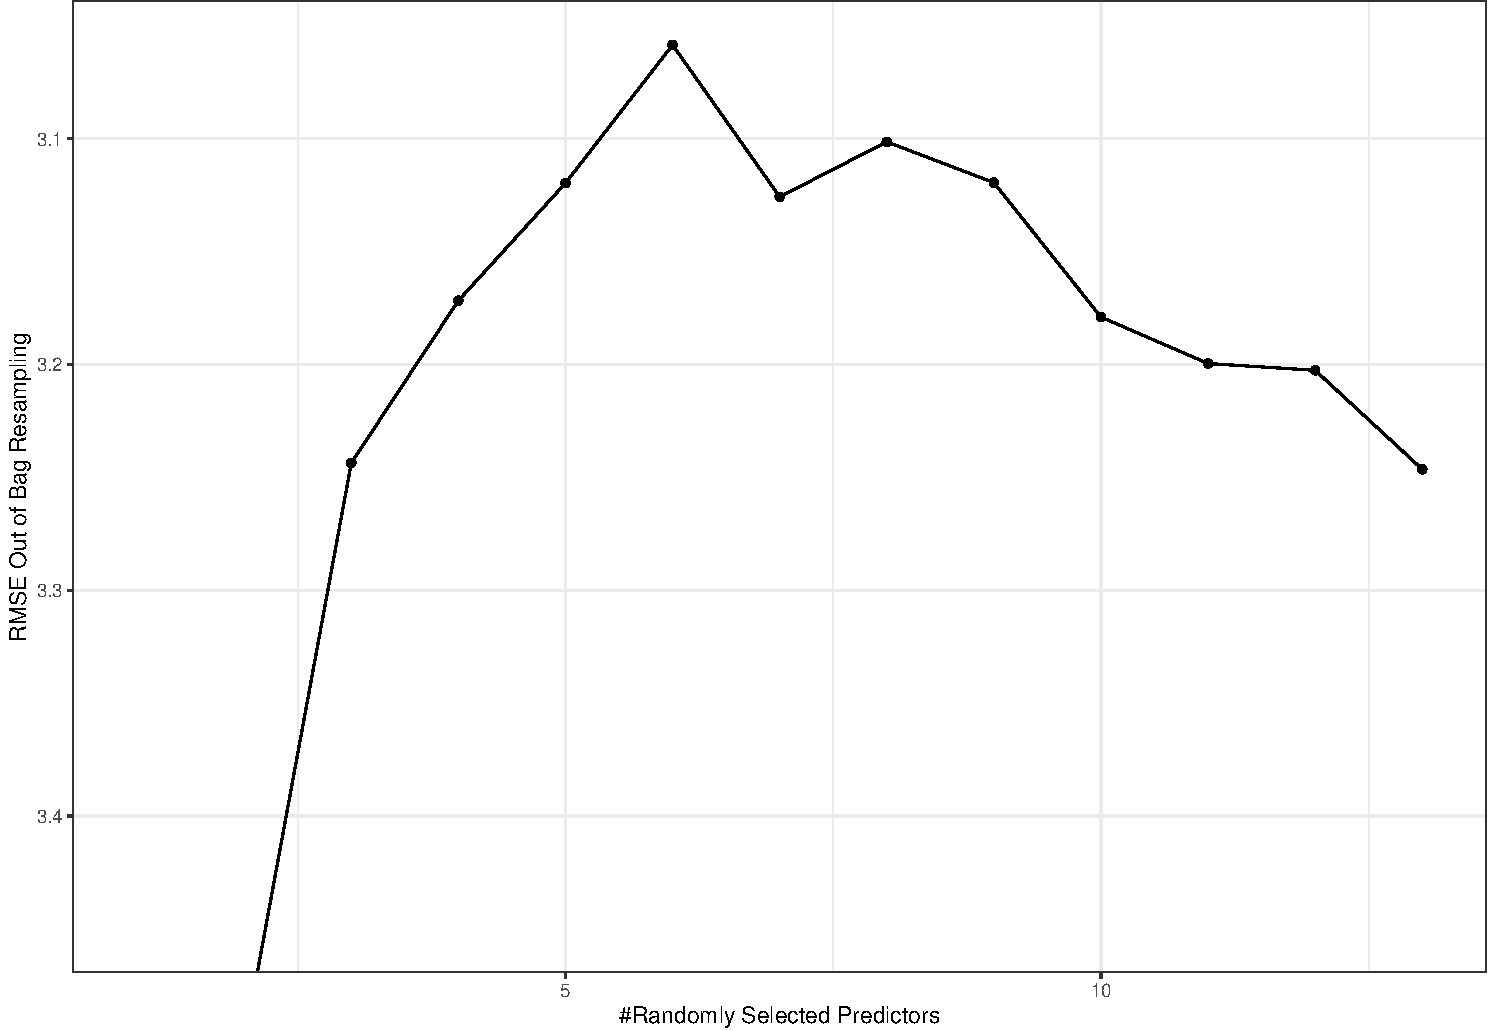
\includegraphics{L7_files/figure-beamer/unnamed-chunk-7-1.pdf}

\begin{Shaded}
\begin{Highlighting}[]
\NormalTok{rf\_tune}\SpecialCharTok{$}\NormalTok{bestTune}
\end{Highlighting}
\end{Shaded}

\begin{verbatim}
##   mtry
## 6    6
\end{verbatim}
\end{block}
\end{frame}

\begin{frame}[fragile]
The R the function \texttt{tune\_bayes} is available in the package
\texttt{tune}, and requires that the analyses is done with a workflow.
Default in the GP is exponential correlation function, but first we try
the Matern.

\begin{Shaded}
\begin{Highlighting}[]
\NormalTok{tree\_rec }\OtherTok{\textless{}{-}} \FunctionTok{recipe}\NormalTok{(medv}\SpecialCharTok{\textasciitilde{}}\NormalTok{crim}\SpecialCharTok{+}\NormalTok{zn}\SpecialCharTok{+}\NormalTok{indus}\SpecialCharTok{+}\NormalTok{chas}\SpecialCharTok{+}\NormalTok{nox}\SpecialCharTok{+}\NormalTok{rm}\SpecialCharTok{+}\NormalTok{age}\SpecialCharTok{+}\NormalTok{dis}\SpecialCharTok{+}\NormalTok{rad}\SpecialCharTok{+}\NormalTok{tax}\SpecialCharTok{+}\NormalTok{ptratio}\SpecialCharTok{+}\NormalTok{black}\SpecialCharTok{+}\NormalTok{lstat, }\AttributeTok{data =}\NormalTok{ Boston)}

\NormalTok{tune\_spec }\OtherTok{\textless{}{-}} \FunctionTok{rand\_forest}\NormalTok{( }\CommentTok{\# parsnip interface to random forests models}
  \AttributeTok{mode=}\StringTok{"regression"}\NormalTok{,}
  \AttributeTok{mtry =} \FunctionTok{tune}\NormalTok{(),}
  \AttributeTok{trees =} \FunctionTok{tune}\NormalTok{(),}
\CommentTok{\#  min\_n = tune()}
\NormalTok{) }\SpecialCharTok{\%\textgreater{}\%}
\CommentTok{\#  set\_mode("regression") \%\textgreater{}\%}
\CommentTok{\#  set\_engine("ranger",objective="reg:rmse") \# errors with ranger}
  \FunctionTok{set\_engine}\NormalTok{(}\StringTok{"randomForest"}\NormalTok{) }\CommentTok{\# randomforest ok}

\NormalTok{tune\_wf }\OtherTok{\textless{}{-}} \FunctionTok{workflow}\NormalTok{() }\SpecialCharTok{\%\textgreater{}\%}
  \FunctionTok{add\_recipe}\NormalTok{(tree\_rec) }\SpecialCharTok{\%\textgreater{}\%}
  \FunctionTok{add\_model}\NormalTok{(tune\_spec)}

\NormalTok{tune\_param }\OtherTok{\textless{}{-}}\NormalTok{ tune\_spec}\SpecialCharTok{\%\textgreater{}\%} 
\NormalTok{  parameters}\SpecialCharTok{\%\textgreater{}\%} 
  \FunctionTok{update}\NormalTok{(}\AttributeTok{mtry=}\FunctionTok{mtry}\NormalTok{(}\FunctionTok{c}\NormalTok{(1L,13L)),}\AttributeTok{trees=}\FunctionTok{trees}\NormalTok{(}\FunctionTok{c}\NormalTok{(100L,500L)))}

\NormalTok{vfold  }\OtherTok{\textless{}{-}} \FunctionTok{vfold\_cv}\NormalTok{(Boston, }\AttributeTok{v =} \DecValTok{5}\NormalTok{)}
\CommentTok{\# then trying BO}
\NormalTok{ctrl }\OtherTok{\textless{}{-}} \FunctionTok{control\_bayes}\NormalTok{(}\AttributeTok{verbose =} \ConstantTok{TRUE}\NormalTok{)}
\NormalTok{bayesres}\OtherTok{\textless{}{-}} \FunctionTok{tune\_bayes}\NormalTok{(tune\_wf,}
    \AttributeTok{resamples =}\NormalTok{ vfold,}
    \CommentTok{\#metrics = rmse,}
    \AttributeTok{corr=}\FunctionTok{list}\NormalTok{(}\AttributeTok{type=}\StringTok{"matern"}\NormalTok{,}\AttributeTok{nu=}\DecValTok{5}\SpecialCharTok{/}\DecValTok{2}\NormalTok{), }
    \CommentTok{\#default in corr\_mat(GPfit) is "exponential" power 1.95}
    \AttributeTok{initial =} \DecValTok{10}\NormalTok{,}
    \AttributeTok{param\_info =}\NormalTok{ tune\_param,}
    \AttributeTok{iter =} \DecValTok{10}\NormalTok{,}
    \AttributeTok{objective=}\FunctionTok{exp\_improve}\NormalTok{(),}
    \AttributeTok{control =}\NormalTok{ ctrl}
\NormalTok{  )}
\FunctionTok{dput}\NormalTok{(bayesres,}\StringTok{"bayesres.dd"}\NormalTok{)}
\end{Highlighting}
\end{Shaded}

\begin{verbatim}
## # A tibble: 10 x 9
##     mtry trees .metric .estimator  mean     n std_err .config              .iter
##    <int> <int> <chr>   <chr>      <dbl> <int>   <dbl> <chr>                <int>
##  1     6   204 rmse    standard    3.16     5   0.231 Iter6                    6
##  2     7   315 rmse    standard    3.17     5   0.257 Iter10                  10
##  3     6   319 rmse    standard    3.19     5   0.254 Iter7                    7
##  4     6   210 rmse    standard    3.19     5   0.262 Iter2                    2
##  5     6   196 rmse    standard    3.20     5   0.252 Preprocessor1_Model~     0
##  6     6   296 rmse    standard    3.22     5   0.256 Preprocessor1_Model~     0
##  7     7   204 rmse    standard    3.22     5   0.287 Iter5                    5
##  8     8   305 rmse    standard    3.23     5   0.280 Preprocessor1_Model~     0
##  9     7   333 rmse    standard    3.23     5   0.271 Iter8                    8
## 10     9   452 rmse    standard    3.24     5   0.283 Preprocessor1_Model~     0
\end{verbatim}

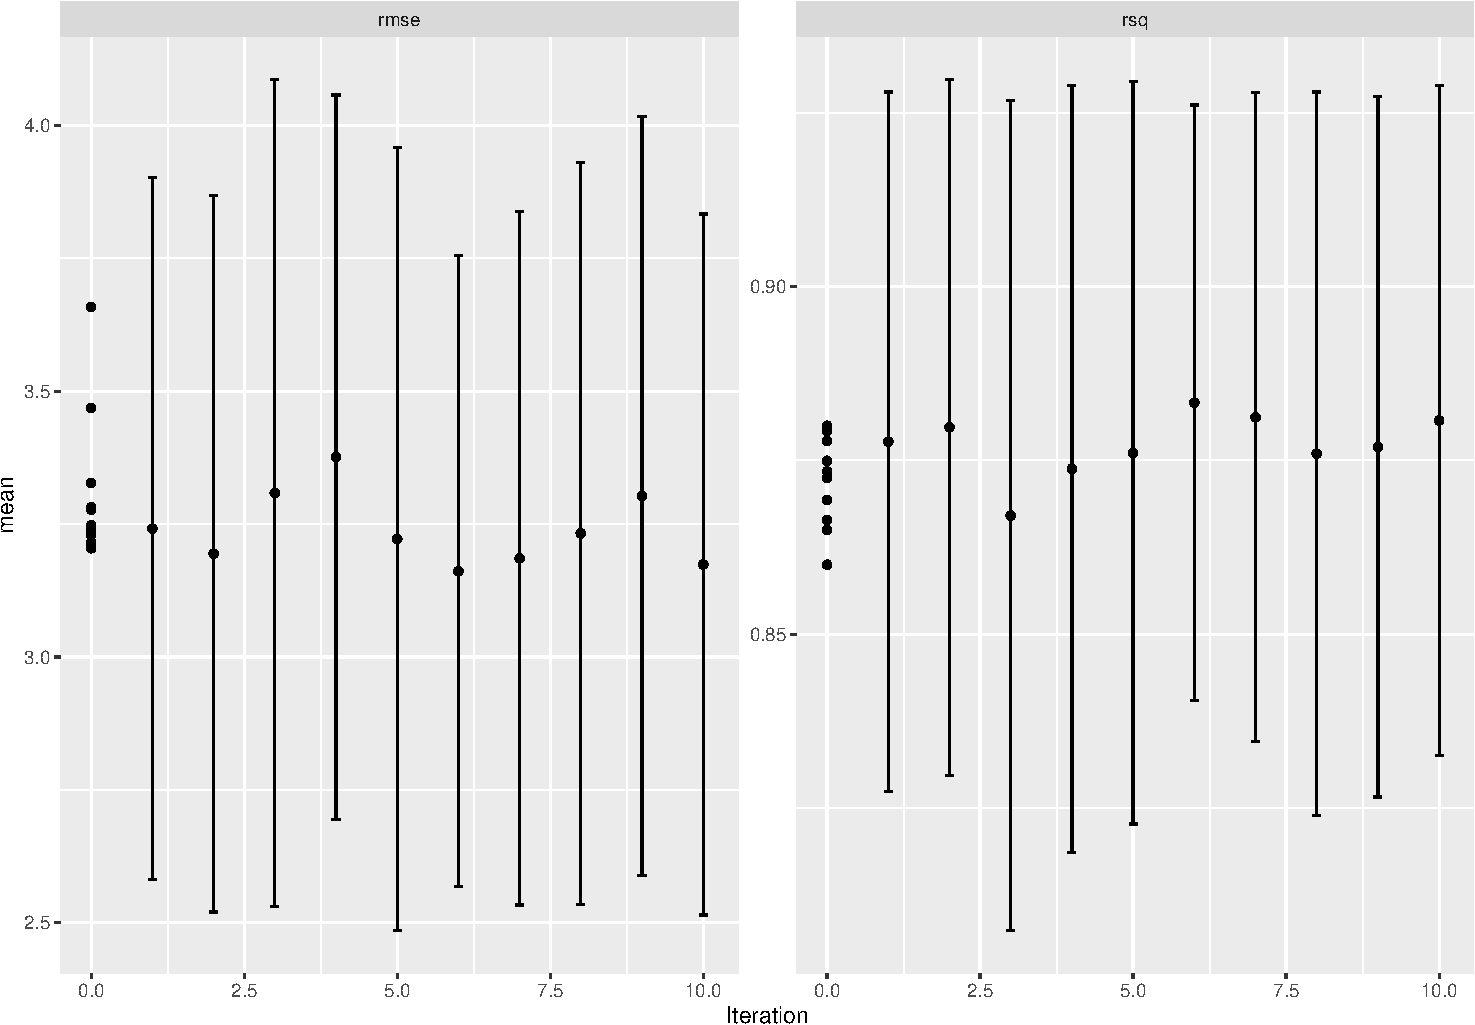
\includegraphics{L7_files/figure-beamer/unnamed-chunk-9-1.pdf}
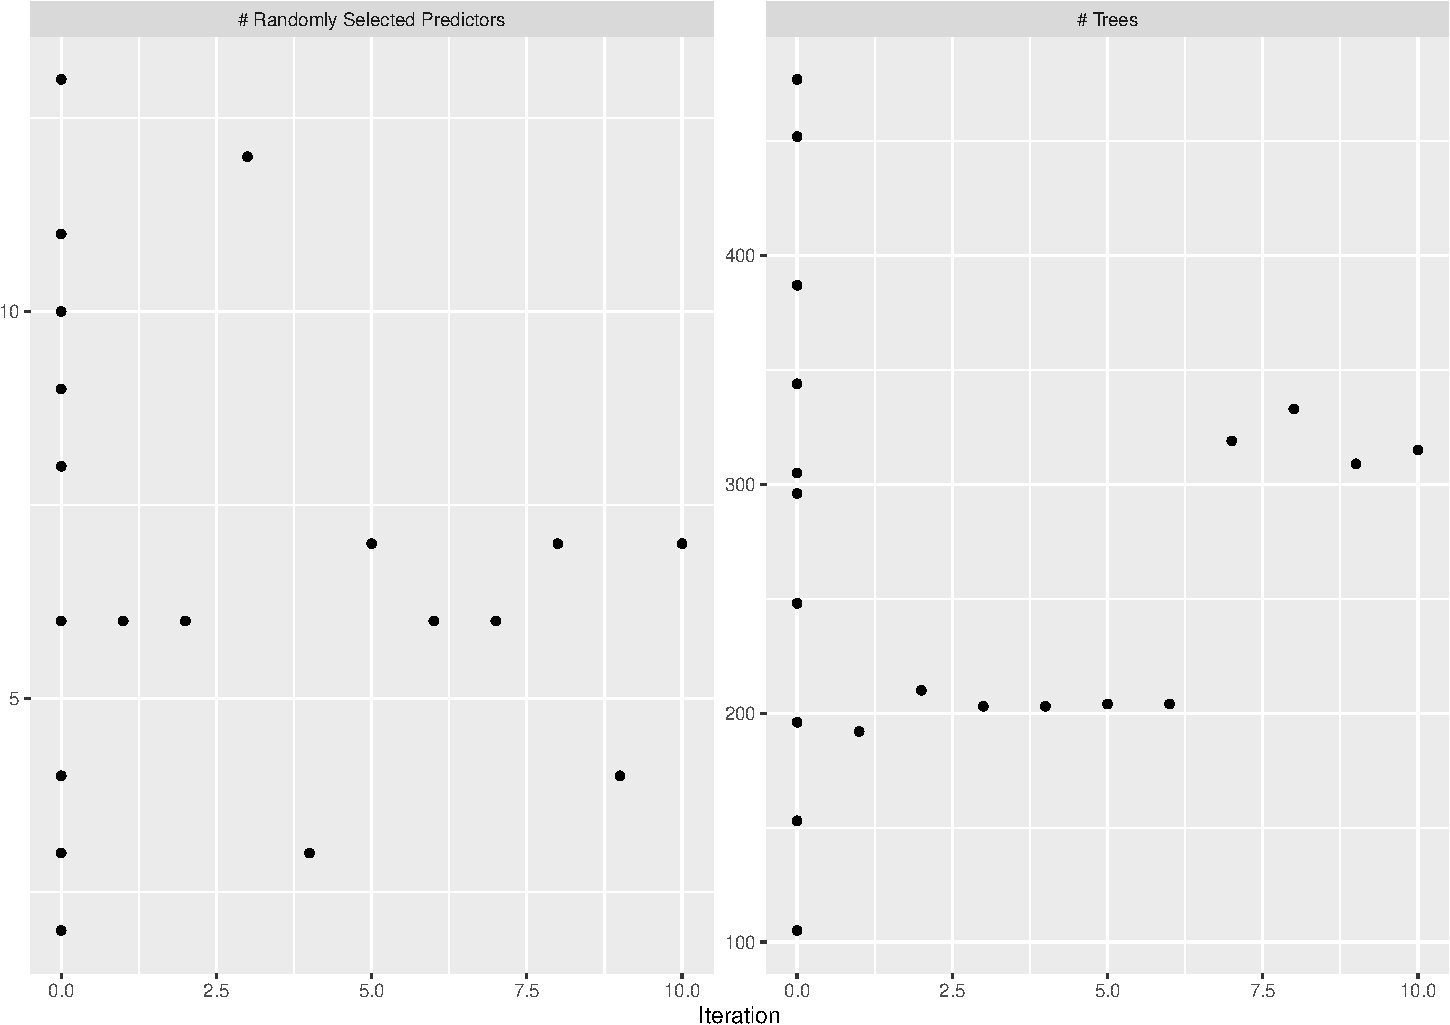
\includegraphics{L7_files/figure-beamer/unnamed-chunk-9-2.pdf}
\end{frame}

\begin{frame}[fragile]
Here we try the default exponential correlation.

\begin{Shaded}
\begin{Highlighting}[]
\NormalTok{bayesres2}\OtherTok{\textless{}{-}} \FunctionTok{tune\_bayes}\NormalTok{(tune\_wf,}
    \AttributeTok{resamples =}\NormalTok{ vfold,}
    \CommentTok{\#metrics = rmse,}
    \CommentTok{\#corr=list(type="matern",nu=5/2), }
    \CommentTok{\#default in corr\_mat(GPfit) is "exponential" power 1.95}
    \AttributeTok{initial =} \DecValTok{10}\NormalTok{,}
    \AttributeTok{param\_info =}\NormalTok{ tune\_param,}
    \AttributeTok{iter =} \DecValTok{10}\NormalTok{,}
    \AttributeTok{objective=}\FunctionTok{exp\_improve}\NormalTok{(),}
    \AttributeTok{control =}\NormalTok{ ctrl}
\NormalTok{  )}
\FunctionTok{dput}\NormalTok{(bayesres2,}\StringTok{"bayesres2.dd"}\NormalTok{)}
\end{Highlighting}
\end{Shaded}

\begin{Shaded}
\begin{Highlighting}[]
\NormalTok{bayesres2}\OtherTok{=}\FunctionTok{dget}\NormalTok{(}\StringTok{"bayesres2.dd"}\NormalTok{)}
\FunctionTok{show\_best}\NormalTok{(bayesres2,}\AttributeTok{n=}\DecValTok{10}\NormalTok{)}
\end{Highlighting}
\end{Shaded}

\begin{verbatim}
## # A tibble: 10 x 9
##     mtry trees .metric .estimator  mean     n std_err .config              .iter
##    <int> <int> <chr>   <chr>      <dbl> <int>   <dbl> <chr>                <int>
##  1     7   311 rmse    standard    3.16     5   0.238 Iter9                    9
##  2     7   122 rmse    standard    3.18     5   0.268 Iter10                  10
##  3     6   101 rmse    standard    3.18     5   0.248 Iter7                    7
##  4     7   102 rmse    standard    3.18     5   0.255 Iter4                    4
##  5     7   249 rmse    standard    3.18     5   0.270 Preprocessor1_Model~     0
##  6     7   500 rmse    standard    3.19     5   0.259 Iter3                    3
##  7     6   278 rmse    standard    3.19     5   0.255 Preprocessor1_Model~     0
##  8     8   113 rmse    standard    3.19     5   0.257 Preprocessor1_Model~     0
##  9     6   164 rmse    standard    3.21     5   0.258 Iter8                    8
## 10     7   101 rmse    standard    3.21     5   0.290 Iter5                    5
\end{verbatim}

\begin{Shaded}
\begin{Highlighting}[]
\FunctionTok{autoplot}\NormalTok{(bayesres2,}\AttributeTok{type=}\StringTok{"performance"}\NormalTok{)}
\end{Highlighting}
\end{Shaded}

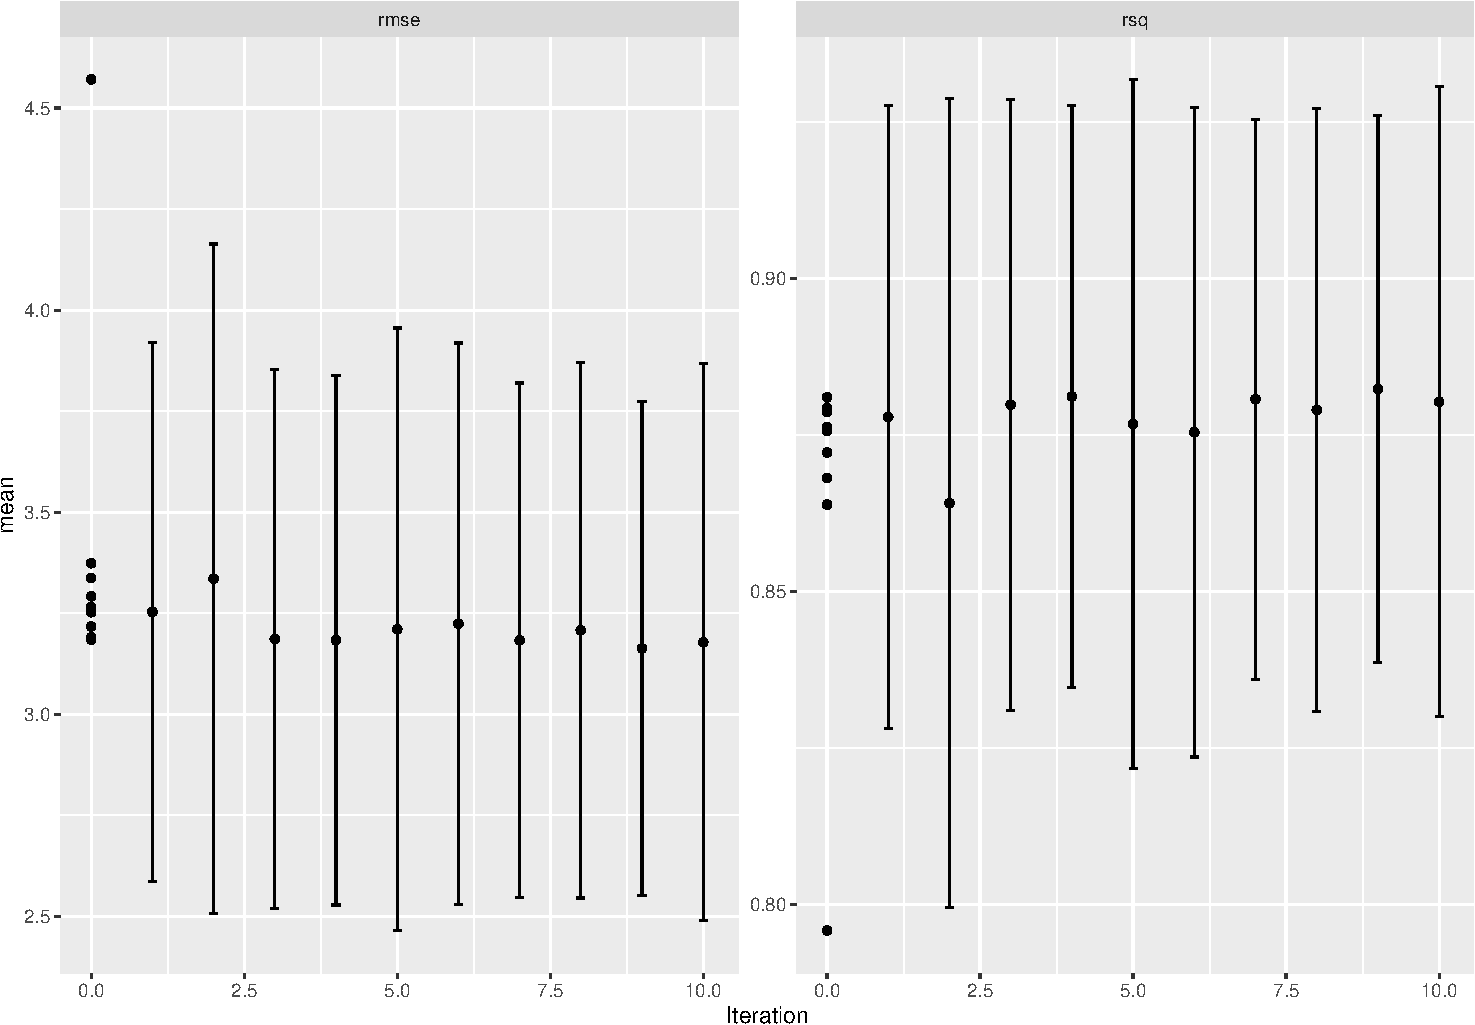
\includegraphics{L7_files/figure-beamer/unnamed-chunk-11-1.pdf}

\begin{Shaded}
\begin{Highlighting}[]
\FunctionTok{autoplot}\NormalTok{(bayesres2,}\AttributeTok{type=}\StringTok{"parameters"}\NormalTok{)}
\end{Highlighting}
\end{Shaded}

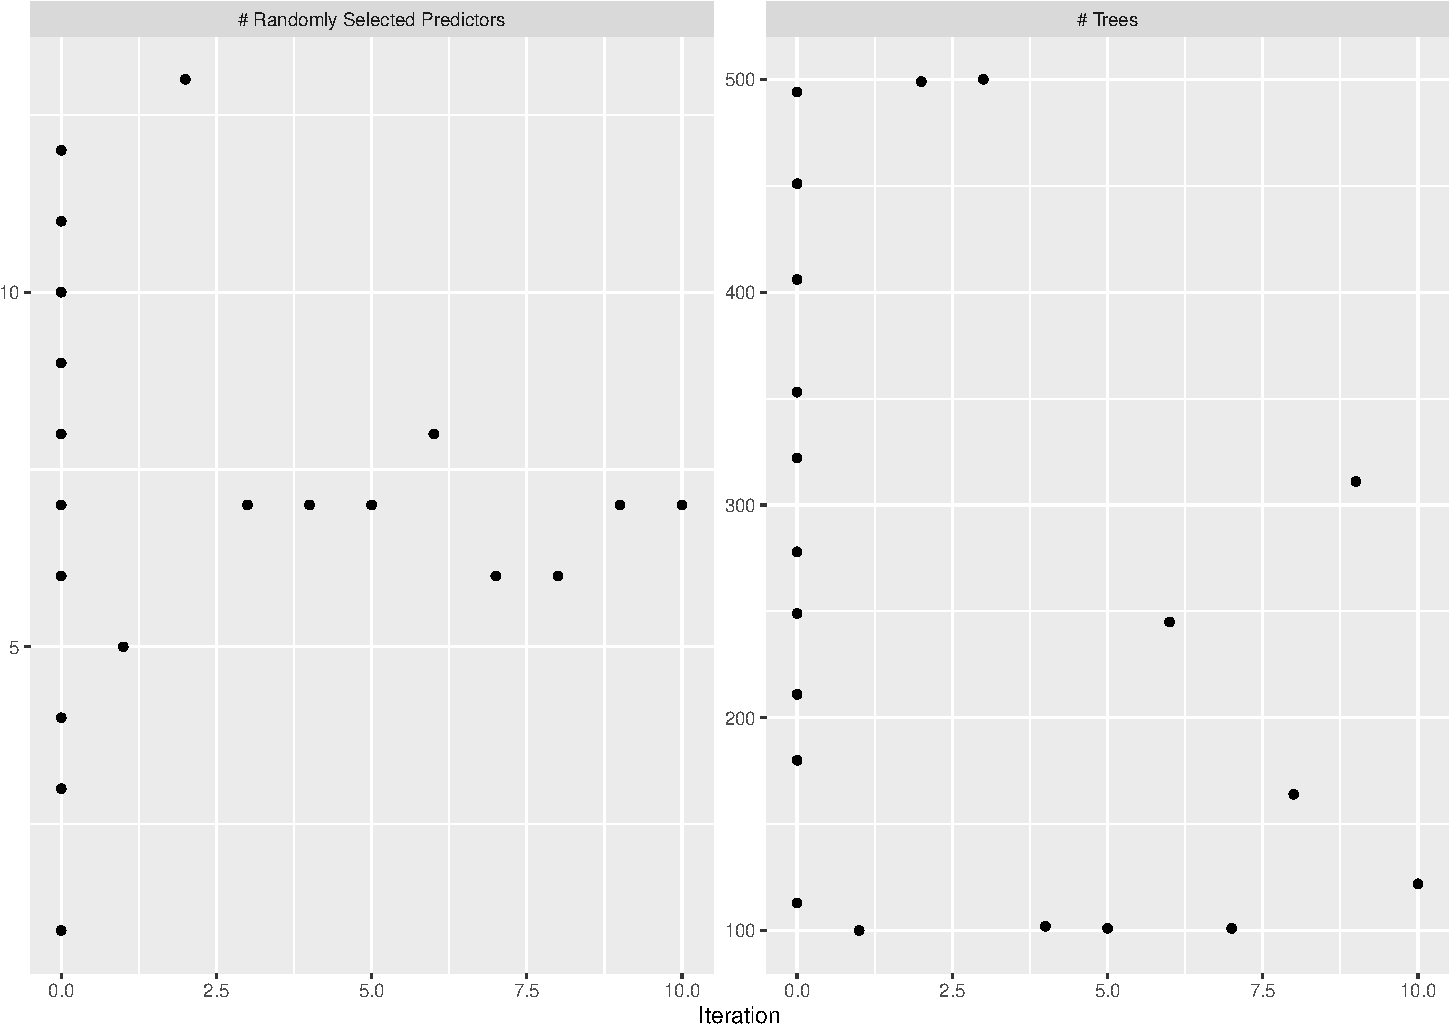
\includegraphics{L7_files/figure-beamer/unnamed-chunk-11-2.pdf}
\end{frame}

\begin{frame}[fragile]
\begin{block}{Suggested software}
\protect\hypertarget{suggested-software}{}
(Frazier 2018, Ch 6)

\begin{itemize}
\item
  R: DiceOptim (on CRAN)
\item
  R: tune\_bayes in \texttt{tune} (also CRAN)
\item
  Python: Spearmint \url{https://github.com/HIPS/Spearmint}
\item
  Python: GPyOpt \url{https://github.com/SheffieldML/GPyOpt}
\item
  Python: GPFlow (Tensorflow) \url{https://github.com/GPflow/GPflow} and
  GPYTorch (PyTorch) \url{https://github.com/cornellius-gp/gpytorch}
\end{itemize}
\end{block}
\end{frame}

\begin{frame}
\begin{block}{Design of experiments and response surface methodology}
\protect\hypertarget{design-of-experiments-and-response-surface-methodology}{}
Article presentation by group 2.

G. A. Lujan-Moreno, P. R. Howard, O. G. Rojas and D. C. Montgomery
(2018): Design of experiments and response surface methodology to tune
machine learning hyperparameters, with a random forest case- study.
Expert Systems with Applications. 109, 195-205.
\end{block}
\end{frame}

\begin{frame}{References}
\protect\hypertarget{references}{}
\begin{block}{Super Learner}
\protect\hypertarget{super-learner-1}{}
\begin{itemize}
\item
  Erin Le Dell (2015):
  \href{https://escholarship.org/uc/item/3kb142r2}{Scalable Ensemble
  Learning and Computationally Efficient Variance Estimation. PhD
  Thesis, University of California, Berkeley.}
\item
  Mark J. van der Laan, Eric C. Polley, Alan E. Hubbard (2007): Super
  Learner, Statistical Applications in Genetics and Molecular Biology,
  6, 1, 25
\item
  Eric C. Polley, Sherri Rose, Mark J. van der Laan (2011): Super
  Learning. Chapter 3 of M. J. van der Laan and S. Rose. Targeted
  Learning, Springer.
\end{itemize}
\end{block}

\begin{block}{Ensembles}
\protect\hypertarget{ensembles}{}
\begin{itemize}
\tightlist
\item
  {[}ELS{]} The Elements of Statistical Learning: Data Mining,
  Inference, and Prediction, Second Edition (Springer Series in
  Statistics, 2009) by Trevor Hastie, Robert Tibshirani, and Jerome
  Friedman.
  \href{https://web.stanford.edu/~hastie/Papers/ESLII.pdf}{Ebook}.
\end{itemize}
\end{block}

\begin{block}{Hyperparameter tuning}
\protect\hypertarget{hyperparameter-tuning}{}
\begin{itemize}
\item
  M. Feurer and F. Hutter (2019). In F. Hutter et al (eds.) Automated
  Machine Learning. The Springer Series on Challenges in Machine
  Learning.
\item
  Jo Eidsvik (2017): Introduction to Gaussian processes, note to
  TMA4265.
\item
  Peter I. Frazier (2018): A tutorial on Bayesian optimization. arxiv
  \url{https://arxiv.org/abs/1807.02811}
\item
  Max Kuhn and Julia Silge Version 0.0.1.9008 (2021-02-15) Tidy
  modelling with R. \url{https://www.tmwr.org/}
\item
  Roger Gosse, University of Toronto: CSC321 Lecture 21: Bayesian
  Hyperparameter Optimization.
  \url{http://www.cs.toronto.edu/~rgrosse/courses/csc321_2017/slides/lec21.pdf}
\item
  Max Kuhn (2020). caret: Classification and Regression Training. R
  package version 6.0-86. \url{https://CRAN.R-project.org/package=caret}
\end{itemize}
\end{block}
\end{frame}

\end{document}
